%Version 2.1 April 2023
% See section 11 of the User Manual for version history
%
%%%%%%%%%%%%%%%%%%%%%%%%%%%%%%%%%%%%%%%%%%%%%%%%%%%%%%%%%%%%%%%%%%%%%%
%%                                                                 %%
%% Please do not use \input{...} to include other tex files.       %%
%% Submit your LaTeX manuscript as one .tex document.              %%
%%                                                                 %%
%% All additional figures and files should be attached             %%
%% separately and not embedded in the \TeX\ document itself.       %%
%%                                                                 %%
%%%%%%%%%%%%%%%%%%%%%%%%%%%%%%%%%%%%%%%%%%%%%%%%%%%%%%%%%%%%%%%%%%%%%

%%\documentclass[referee,sn-basic]{sn-jnl}% referee option is meant for double line spacing

%%\documentclass[lineno,sn-basic]{sn-jnl}% Basic Springer Nature Reference Style/Chemistry Reference Style

%%\documentclass[pdflatex,sn-basic]{sn-jnl}% Basic Springer Nature Reference 
 
\documentclass[pdflatex, sn-nature]{sn-jnl}% Style for submissions to Nature Portfolio 

%%%% Standard Packages
\usepackage{graphicx}%
\usepackage{multirow}%
\usepackage{amsmath,amssymb,amsfonts}%
\usepackage{amsthm}%
\usepackage{mathrsfs}%
\usepackage[title]{appendix}%
\usepackage{xcolor}%
\usepackage{textcomp}%
\usepackage{manyfoot}%
\usepackage{booktabs}%
\usepackage{algorithm}%
\usepackage{algorithmicx}%
\usepackage{algpseudocode}%
\usepackage{listings}%
\usepackage{gensymb} %added by V. Van der Meersch
\usepackage{comment} %added by V. Van der Meersch
 \usepackage{textcomp} %added by V. Van der Meersch
 \newcommand{\textappr}{\raisebox{0.5ex}{\texttildelow}} %added by V. Van der Meersch

%%%%

%%%%%=============================================================================%%%%
%%%%  Remarks: This template is provided to aid authors with the preparation
%%%%  of original research articles intended for submission to journals published 
%%%%  by Springer Nature. The guidance has been prepared in partnership with 
%%%%  production teams to conform to Springer Nature technical requirements. 
%%%%  Editorial and presentation requirements differ among journal portfolios and 
%%%%  research disciplines. You may find sections in this template are irrelevant 
%%%%  to your work and are empowered to omit any such section if allowed by the 
%%%%  journal you intend to submit to. The submission guidelines and policies 
%%%%  of the journal take precedence. A detailed User Manual is available in the 
%%%%  template package for technical guidance.
%%%%%=============================================================================%%%%

%\jyear{2021}%

\raggedbottom
\unnumbered% uncomment this for unnumbered level heads

\begin{document}

\title[Article Title]{Temporary titles: Causal relationships ensure model robustness  / Causal relationships improve model projections reliability}

\author*[1]{\fnm{Victor} \sur{Van der Meersch}}\email{victor.vandermeersch@cefe.cnrs.fr}
\author[2]{\fnm{Edward} \sur{Armstrong}}
\author[3]{\fnm{Frédérik} \sur{Saltré}}
\author[1]{\fnm{Florent} \sur{Mouillot}}
\author[4]{\fnm{Anne} \sur{Duputié}}
\author[5]{\fnm{Cristophe} \sur{Randin}}
\author[6]{\fnm{Hendrik} \sur{Davi}}
\author[1]{\fnm{Isabelle} \sur{Chuine}}

\affil[1]{\orgdiv{CEFE}, \orgname{Université de Montpellier, CNRS, EPHE, IRD}, \orgaddress{\city{Montpellier}, \country{France}}}
\affil[2]{\orgdiv{Dept. of Geosciences and Geography}, \orgname{University of Helsinki}, \orgaddress{\city{Helsinki}, \country{Finland}}}
\affil[3]{\orgdiv{Global Ecology}, \orgname{College of Science and Engineering, Flinders University}, \orgaddress{\city{Adelaide}, \country{Australia}}}
\affil[4]{\orgdiv{UMR 8198-EEP-Evo-Eco-Paleo}, \orgname{Université de Lille, CNRS}, \orgaddress{\city{Lille}, \country{France}}}
\affil[5]{\orgdiv{Dept. of Ecology and Evolution}, \orgname{Univ. Lausanne}, \orgaddress{\city{Lausanne}, \country{Switzerland}}}
\affil[6]{\orgdiv{URFM}, \orgname{INRAE}, \orgaddress{\city{Avignon}, \country{France}}}

\abstract{The recent acceleration of global climate warming has urged the need for reliable projections of species distribution and ecosystem functioning. However, little is known about which modelling approach has the potential to provide the most reliable projections under novel environmental conditions. Here, we used multiple types of models, from correlative to process-based with their hybrids, to hindcast the range shift of five tree species across Europe over the last 12,000 years and evaluated their predictions against fossil pollen records. While projections of all models are less reliable moving back in the past, we show that the  performance of correlative models (CSDMs) decreases \textappr2.5 times faster than that of process-based models (PBMs) when climatic dissimilarity rises. We further find that inverse calibration of PBMs, using the same data as CSDMs, does not affect their reliability. These findings highlight the importance of considering causal relationships to ensure model robustness, and provide a promising framework to promote process-based approaches to deliver more accurate projections in the future.}

\keywords{Species range shift, ecological modelling, model transferability, tree species}

\maketitle

\newpage

% CUTE BABY: we need reliable projections of the distribution of species

% WEREWOLF: models perform less well under different conditions than those in which they were built/calibrated... and in addition, in the future, climatic conditions are expected to be very different
% And we don't know which model will be the most robust! :-( 

% SILVER BULLET: through this comparison in the Holocene, we highlight that it is necessary to model cause-and-effect relationships describing the abilities of species to survive/grow/reproduce in various env conditions
% and that inverse calibration using large-scale data may serve as an important step to facilitate the use of process-based models in a very near future :-) :-) :-) yippee!

\section{Main}
  
The complexity of ecosystems functioning makes model simulations key to understanding how climate impacts ecosystems over time. As the demand for reliable projections is increasing, the systematic evaluation of model performance should be one of the main concerns of modellers. Such evaluation indeed remains critical to build confidence in model projections, and plays a crucial role in providing credible information for decision makers and stakeholders \cite{Dawson2011, Mouquet2015, Pacifici2015}.

The most straightforward approach to evaluate model reliability is to compare their predictions to observations from previous periods. Reproducing the past can be seen as a requisite condition to reliably forecast the future. While exact matches to expected 21\textsuperscript{st}-century climatic conditions do not exist in historical records \cite{Burke2018}, the dissimilarity between 20th and 21th century median conditions fall within the range of dissimilarity between 21th century and the 12kyr (\hyperref[climatic_dissimilarity]{Fig. 1}). Hindcasting exercises can thus provide insights whether models capture, implicitly or explicitly, the essential processes required to provide reliable projections in conditions significantly different from the present. By looking far in the past, paleo-archives have indeed proven to offer a unique framework to understand long-term both climate and biodiversity dynamics \cite{Fordham2020} and to test model transferability  \cite{Braconnot2012, Maguire2015}.

\begin{figure}[ht]
\centering
\hspace*{-0.6in}
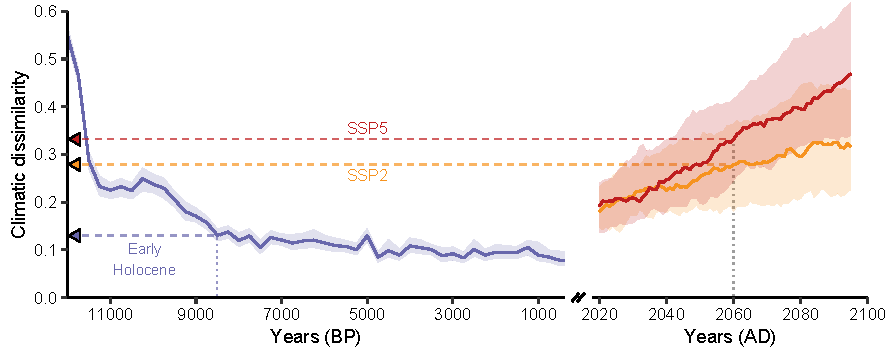
\includegraphics[scale=1]{climatic_dissimilarity.pdf}
\caption{\textbf{Evolution of climatic dissimilarity under past (12k-500 yr BP) and future (2005-2100) climate changes, relative to 1901-2000}. Climatic dissimilarity is computed as 1-Sørensen similarity between bootstrapped climatic hypervolumes. Lines represent median dissimilarity, shaded areas represent 90\% confidence intervals. Blue corresponds to paleoclimate based on HadCM3B model. Yellow and red correspond to SSP245 and SSP585 scenarios, each based on 30 models. Blue triangle on y-axis indicates the limit between Early Holocene (before 8200BP) and Late-Middle Holocene (after 8200BP). Yellow and red triangles indicate the expected level of climatic dissimilarity in 2060 for SSP245 and SSP585 scenarios. Note that the x-axis scale changes across past and future panels.}\label{climatic_dissimilarity}
\end{figure}

Models commonly reveal a decrease of their ability to provide accurate projections of either climate \cite{Harrison2015} or species/biomes distribution \cite{Veloz2012, Pearman2008, Roberts2012, Foley2013} in the distant past, i.e. spanning several millennia, using paleoclimate reconstructions and fossil records. This calls for caution when interpreting their projections in climatic conditions that differ significantly from the present \cite{Maguire2016}, and this is all the more important since no-analogue climatic conditions are forecasted to become more common \cite{Williams2007}, potentially compromising the reliability of model projections for the 21st century \cite{Fitzpatrick2018}.

Regarding species geographical distribution, most studies have focused on correlative models (CSDMs, also called environmental niche models), which infer statistical relationships between observations of species occurrences and environmental predictors \cite{Dormann2012}.  Other models, called process-based models (PBMs), are built upon explicit causal relationships determined experimentally between on one hand physiological, ecological and demographic processes, and on the other hand environmental drivers \cite{Dormann2012}. Because they describe causal relationships, they are expected to enhance our ability to understand and predict species responses to climate change and to provide more robust projections in novel conditions \cite{Evans2012, Singer2016}. Projections of PBMs in future climatic conditions have been so far systematically more conservative than those of CSDMs \cite{Morin2009, Cheaib2012, Gritti2013}. However, despite the growing interest for PBMs in predictive ecology \cite{Connolly2017, Urban2016, Pilowsky2022}, very few studies have gone beyond qualitative comparisons between the models and compared thoroughly their performance, for example using virtual species \cite{Zurell2016}, exotic species in native and newly colonized areas \cite{Higgins2020}, or in the recent past \cite{Fordham2018}. While PBMs have shown their usefulness for paleoecological studies \cite{Saltre2013, Ruosch2016, Schwoerer2014}, the extent to which they can provide more reliable predictions than correlative models in very different climatic conditions from present remains unknown as well as the reasons why they could do so \cite{UribeRivera2022, Briscoe2019}. Such assessment has become a very high priority to guide more efficiently biodiversity management plans \cite{Pacifici2015}.

Here, we address these shortcomings by using multiple CSDMs and PBMs to simulate paleodistributions of emblematic tree species of Europe at a high-temporal resolution. We also incorporated species migration in the simulations and evaluated model performance against fossil pollen records. We extend this analysis by including hybrid models in the comparison, i.e. PBMs calibrated in the same way as CSDMs (inverse calibration using species occurrence data and a novel type of algorithm, \hyperref[methods]{Methods} and \citep{VanderMeersch2023}). Encompassing the entire spectrum of models, from correlative models to process-based models and their hybrid data-driven counterparts, allowed us identifying the key features necessary for building robust models. We additionally quantified the dissimilarity between past climatic conditions and historical conditions (in terms of hypervolume overlap, \hyperref[methods]{Methods}) to investigate its effects on model performance.
Globally, we find that the predictive performance of all models decreased moving back in time and in increasingly novel climates, but PBMs overall maintained a better performance and a higher transferability in distant climatic conditions. We also find that inverse calibration may help improve PBMs performance without compromising their long-term transferability.

\begin{figure}
\centering
\vspace*{-0.6in}
\hspace*{-0.35in}
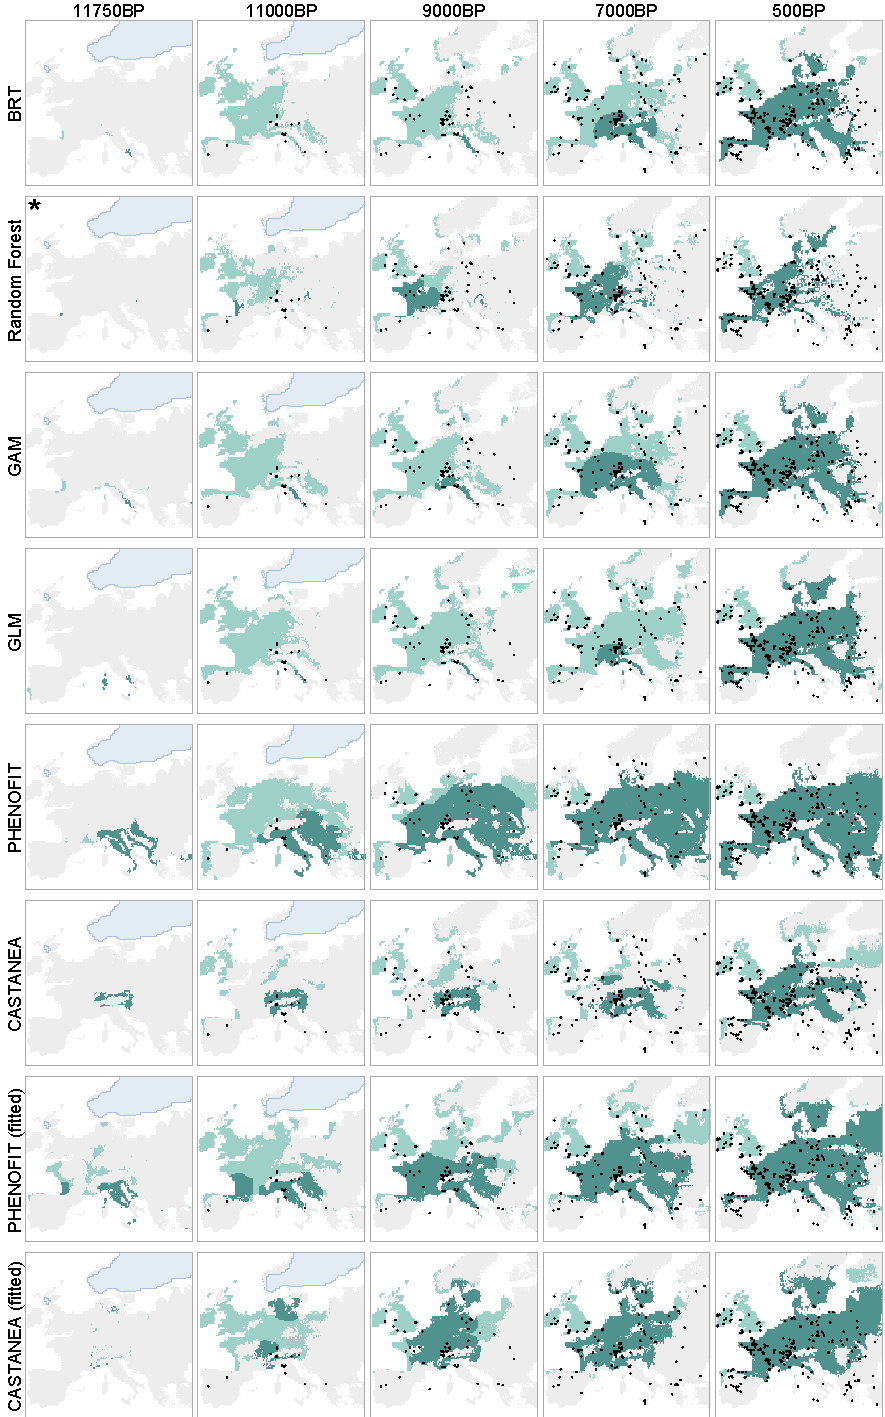
\includegraphics[scale=0.95]{quercus_deciduous_simulations.pdf}
\caption{\textbf{Example of paleosimulations obtained with the eight models used in this study for deciduous oaks.} Four first rows correspond to the four correlative models (boosted regression tree, down-sampled random forest, generalized additive model, generalized linear model with lasso regularization). Four last rows correspond to two different versions (expert calibration and inverse calibration) of two process-based models (PHENOFIT and CASTANEA). Light green area is the modelled suitable area, dark green area is the colonized area (after migration). Light blue represents the ice sheet extent. Black dots are deciduous oak fossil pollen occurrences. Model for which migration started at 117500 BP rather than 12000 BP is marked with an asterisk. "BP" stands for "before present" (1950).}\label{quercus_migration}
\end{figure}



\renewcommand\labelitemi{{\boldmath$\cdot$}}
\begin{itemize}
\setlength\itemsep{1em}
\item \emph{Models hindcast skills}\par
\item Unsurprisingly, all models showed a decrease of their performance by moving further away in the past, in more novel climatic conditions (\hyperref[past_performance]{Fig. 3a}). Without migration, model ability to predict fossil pollen occurrence were similar (Extended Data Fig. 11), with an average Sørensen index decrease of $-0.214\pm0.0153$ (paired Wilcoxon-test, $P<0.0001$) and TSS decrease of $-0.146\pm0.0421$ (paired Wilcoxon-test, $P=0.00093$) between Late-Middle Holocene (after 8200BP) and Early Holocene (before 8200BP).  When accounting for migration since 12.000BP, novel climatic conditions had a stronger impact on the predictions of CSDMs (slope of Beta regression, $-13.2$, 95\% CI $[-15.9, -10.5]$) than those of fitted PBMs ($-7.24$, 95\% CI $[-10.4, -4.16]$) and expert PBMs ($-5.92$, 95\% CI $[-8.96, -2.86]$). CSDMs and fitted PBMs were significantly better at predicting tree distribution in the near past (Late-Middle Holocene) than expert PBMs (pairwise Conover-Iman tests, respectively $P=0.018$ and $P=0.00046$, \hyperref[past_performance]{Fig. 3c}), reflecting their closer fit to current species distributions, whereas both expert and fitted PBMs performed better in the Early Holocene (pairwise Conover-Iman tests, both $P<0.0001$, \hyperref[past_performance]{Fig. 3c}). Expert PBMs proved to have on average a better transferability (model capacity to maintain its performance in changing conditions \cite{UribeRivera2022}) and maintained a good performance despite a high level of climatic dissimilarity (\hyperref[past_performance]{Fig. 3b}). As they are not calibrated using current species distribution-climate relations contrary to fitted PBMs and CSDMs, they might be less sensitive to novel climatic regimes. Model performance varied depending on the species considered, and exhibited both similarities and differences in performance across time (Extended Data Fig. 10). More specifically, models exhibited the same overall performance decrease against \emph{Fagus} pollen records, whereas CSDM performance decline was substantially faster than expert and fitted PBMs for deciduous \emph{Quercus}. All models show poor predictions of evergreen \emph{Quercus} distribution even in the recent past compared to other species, especially CSDMs which failed to predict its presence along the Atlantic coast (Extended Data Fig. 7).

\item Most of the variability among models performance is due to the differences in their projections during the late Pleistocene-Early Holocene. This period  corresponds to a global deglacial warming which last a few centuries and occurred after the cooling of the Younger Dryas interval  (Extended Data Fig. 1). This rapid warming episod explains the rapid decrease of climatic dissimilarity to present after 12000BP (\hyperref[climatic_dissimilarity]{Fig. 1}). Since the migration model was identical across all simulations, differences of performance between models across the Holocene very much depend on their ability to predict the potential refugia of the species during the Early Holocene. For example, some models were not able to predict evergreen \emph{Quercus} refugia in Southern Spain, and thus miss an important migration route and fail predicting their presence in vast areas in the Late Holocene (Extended Data Fig. 7). Both types of PBMs, fitted and expert, were more performant than CSDMs to predict species recolonisation dynamics in the Early Holocene because they predicted more accurate refugia, i.e. starting points for the migration cellular automaton model (\hyperref[quercus_migration]{Fig. 2} and \hyperref[methods]{Methods}). As PBMs, either fitted or expert, describe the response of ecophysiological processes to a wide range of environmental conditions, they may provide a better estimation of the conditions where species could have survived 12000 years ago, in more distant climates. Note that migration also sometimes undermined models performance. For example all models failed to predict deciduous \emph{Quercus} in the British Isles before the Early Holocene sea level rise and the opening of the Strait of Dover (\hyperref[quercus_migration]{Fig. 2} and \cite{Smith2011}), even though the land-sea mask changed throughout the simulations. We cannot assert whether this could be due to misrepresented very long-distance dispersion of seeds, e.g. by humans or jays, across major dispersal barrier, or a misprediction of more northern refugia.


\begin{figure}[ht]
\centering
\hspace*{-0.8in}
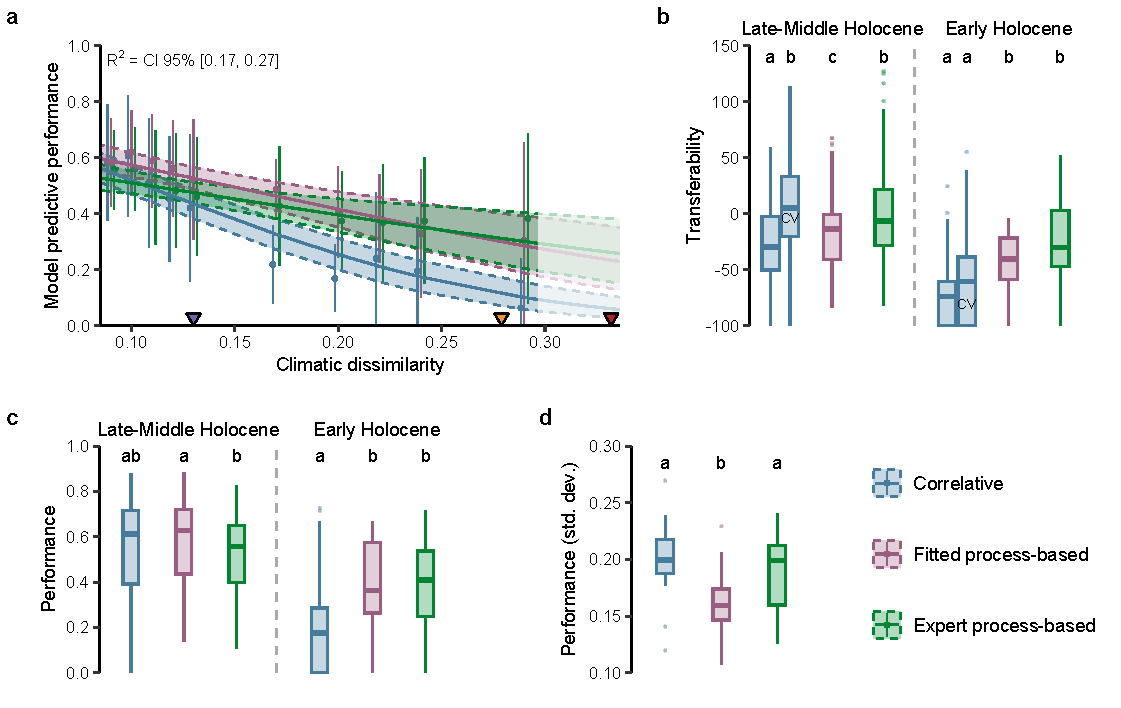
\includegraphics[scale=0.9]{past_performance.pdf}
\caption{\textbf{Performance of correlative models, fitted process-based models (inverse calibration using occurrence data) and expert process-based models (classical calibration) against Holocene paleoecogical evidence (fossil pollen) for 4 tree genera (\emph{Abies}, \emph{Fagus}, \emph{Quercus} deciduous and \emph{Quercus} evergreen).} \textbf{(a)} Bayesian beta regression of model predictive performance (Sørensen index) against climatic dissimilarity relative to 1901-2000 (1-Sørensen similarity between climatic hypervolumes). Shaded areas represent 2.5\% and 97.5\% quantiles of the posterior predictive distribution. Points represent the average model performance (and lines the standard deviation) grouped by similar level of climatic dissimilarity . Blue triangle on x-axis indicates the limit between Early Holocene (before 8200BP) and Late-Middle Holocene (after 8200BP). Yellow and red triangles indicate the expected level of climatic dissimilarity in 2060 for SSP245 and SSP585 scenarios. Panel \textbf{(b)} shows the difference of transferability (relative change in model performance between projected period and calibration period) across models. "CV" stands for "cross-validation", when correlative extrapolation errors (in calibration period) were assessed using a block cross-validation method. Panels \textbf{(c)} and \textbf{(d)} show the difference in performance (Sørensen index) and variability in performance (standard deviation of Sørensen index) across models. The grouping letters represent the multiple comparisons with pairwise Conover-Iman tests. }\label{past_performance}
\end{figure}

\item \emph{Can model performance in the past give a hint of their performance in the future?}\par
\item Although hindcast exercices allow validating models in very different conditions from those used for their calibration, they do not guarantee their validity in the future. They only provide an evaluation of model consistency with some observations, which does not demonstrate that the model is an accurate representation of reality \cite{Oreskes1994}. Acknowledge these uncertainties is as important as to make the predictions themselves \cite{Beale2012} and contributes to the public trust in scientists \cite{Berkhout2010}. Despite different future projections among global climate models (Extended Data Fig. 2), the rate of anthropogenic climate change is challenging the reliability of both CSDMs and PBMs. The occurrence of novel climates is predicted to increase (\cite{Williams2007} and \hyperref[climatic_dissimilarity]{Fig. 1}), and should be carefully considered when models are intended to be used by managers and to guide policies.
\item The scarcity and strong uncertainties of pollen data prevented us from assessing model performance prior 11.5kyr BP although our simulations started at 12kyr BP, which is unfortunate since climate dissimilarity sharply increases and doubles from 11.5 to 12 kyr BP. Nevertheless, the accuracy of the starting point of the simulations at 12kyr BP plays a major role in the evaluation of models performance across the Holocene (Extended Data Fig. XX).  From 11500BP onwards, climatic dissimilarity varies between 0.29 and 0.08, a level equivalent to what we might experience in the first half of the 21st century (\hyperref[climatic_dissimilarity]{Fig. 1}). However, future climatic conditions will shift in a different direction from what happened during Holocene (Extended Data Fig. 3), which prevent us from making a solid quantification of models projections uncertainty. Moreover, tree colonization dynamics will likely be very different in the future: it will not only occur from few refugia, and direct anthropogenic factors, such as sylvicultural practices and assisted population migration, will shape the composition of forests. Nevertheless, our results still serve as an important step towards an assessment of model transferability and prediction uncertainties, not solely based on the model's own prediction dispersion. Without being able to estimate how models will perform in 2100, we can still assess that predictions of PBMs, either fitted or expert, should be more reliable up to 2060 according to the scenario SSP245 (\hyperref[past_performance]{Fig. 3a}). However, as soon as 2060, the level of climate dissimilarity predicted by the scenario SSP585 will exceed the range investigated in this study, and there is no guarantee that any model will be robust in even more distant climate. 

\item \emph{Scaling-up process-based models}\par
\item Our simulations reveal that fitted PBMs have an intermediate behaviour between CSDMs and expert PBMs. In Late-Middle Holocene, their performance is equivalent to CSDMs (pairwise Conover-Iman test, $P=0.054$, \hyperref[past_performance]{Fig. 3c}), which is consistent with the fact that both types of models use the same data for their calibration, i.e species present distribution, and the fact that climate conditions did not change drastically along this period compared to present (\hyperref[climatic_dissimilarity]{Fig. 1}). Further back in time (Early Holocene), while affected by the increase in climate dissimilarity like other models, the performance and the transferability of fitted PBMs is similar to those of expert PBMs and higher than CSDMs (\hyperref[past_performance]{Fig. 3bc}). By explicitly representing causal relationships, both fitted and expert PBMs thus seem to be less affected by the increase in climatic dissimilarity, where species-climate correlations assumed in CSDMs may not hold true.  In addition to allowing separate investigation of the effects of environmental stresses on tree survival, growth, and reproduction, causal relationships are thus critical to ensure higher model robustness in more novel climatic conditions. 
\item Fitted PBMs thus seem to borough strengths from both approaches, i.e. describe causal relationships between environmental conditions and species performance and precise estimation of parameter values. The differences between expert and fitted version of PBMs in the Middle-Late Holocene pinpoint some deficiencies in expert parametrisation which is tedious and requires to combine various methods to cope with both the scarcity of data for each ecophysiological process modelled and sometimes unmeasurable parameters (e.g. \citep{DeCaceres2023}).  Some parameters in these relations can be measured directly, and exhibit little variability across a species range (e.g. water potential leading to 50\% of vessels embolism). However, the measurement of parameters in controlled conditions does not necessarily guarantee their external validity \emph{in natura} \cite{Asse2020} where much more factors, not represented in laboratory conditions, can also affect the process modelled (but see \cite{Satake2013}). Other parameters are either highly variable because of local adaptation,  difficult-to-measure or so far unmeasurable (e.g. bud dormancy break date). Therefore, expert PBMs can suffer from uncertainties entailed in the measurements of some of their parameters, and from spurious data specific to few locations which do not represent sufficiently well all the conditions the species can experience all over its range. For all these reasons, inverse calibration can provide a valuable opportunity to estimate the values of PBMs parameters especially difficult to estimate otherwise. However, inverse calibration using only occurrence data is far from being perfect \cite{VanderMeersch2023}, and is only a first step towards a better parametrization of PBMs. Given ongoing improvements to computational methods and newly available observations at a global scale (such as remote sensing LiDAR data), there is an avenue for the extensive use of process-based models to provide both realistic and reliable projections in future climates.

\item \emph{Conclusion?}\par
% CSDMs can teach us process-based model-building strategies that allow for the propagation of errors, and allow to separate uncertainty sources within model (imprecise parameters, input data, ...) ?
% Hybrid approach: "\emph{Interest to balance biological realism and flexibility in model building with limited knowledge}" (IPBES, chapter 4) => citation à rajouter peut-être qq part
% idea in Evans 2012: forecast need to be realistic and need to be reliable in novel conditions \cite{Evans2012} (two conditions) + In climatological research, forecasting is done using process-based models! 
\item The unique multi-model comparison across the Holocene provided by this study suggests that our understanding of ecophysiological processes embedded into process-based models can provide a real advantage as compared to empirical relations used in CSDMs to provide reliable projections in the upcoming decades. However, data availability places limits on how a model can be parameterized, and could explain the difficulty to extrapolate expert parameters to global impact studies. Fitted PBMs may overcome this problem by using more data at a larger geographical scale, while keeping the predictive strength of causal relationships.
\end{itemize}

\backmatter

\section*{Data and code availability}

Simulation outputs, together with the code to reproduce the analysis and figures in this study, are available on GitHub at \url{https://github.com/vvandermeersch/past_robustness}.

\section*{Acknowledgments}

We acknowledge the support and computing resources of GenOuest and TGCC-CEA. V.V. was supported by a GAIA doctoral school PhD Fellowship.

\section*{Ethics declarations}

The authors declare no competing interests.

%%===========================================================================================%%
%% If you are submitting to one of the Nature Portfolio journals, using the eJP submission   %%
%% system, please include the references within the manuscript file itself. You may do this  %%
%% by copying the reference list from your .bbl file, paste it into the main manuscript .tex %%
%% file, and delete the associated \verb+\bibliography+ commands.                            %%
%%===========================================================================================%%

\bibliography{robustness_bibliography}% common bib file
%% if required, the content of .bbl file can be included here once bbl is generated
%%\input sn-article.bbl


%%Online only Methods should be presented in a separate section after the end of the main text
%% and reference list

\section{Online methods}\label{methods}

\subsection{Correlative and process-based models}\label{models}

Two process-based models were used in this study. 
PHENOFIT simulates the fitness of an average adult tree using daily meteorological data, soil water holding capacity and species-specific parameters \cite{Chuine2001}. It estimates fitness components (survival and reproductive success) by simulating the precise phenology (dates of leaf unfolding, flowering, fruit maturation, leaf senescence) and damages caused by abiotic stress (frost, drought) which effects depend on their occurrence relatively to the development stages of the different organs. It has been used for several North American and European species \cite{Morin2007, Saltre2013, Duputie2015, Gauzere2020}. The model has \textappr30 parameters. 
CASTANEA simulates carbon and water cycles of an average adult tree by simulating many processes such as photosynthesis, stomatal opening, maintenance and growth respiration, transpiration and carbon allocation  \cite{Dufrene2005}. It has used to predict carbon and water budgets of several European species \cite{Davi2006, Delpierre2012, Davi2017}. 
The model has \textappr80 parameters. 
Both models require daily meteorological variables and soil characteristics. Two versions of both models were employed: one was calibrated with expert knowledge and statistical inference using observations and measurements of the processes modelled (version called \emph{expert}), and a second one calibrated using species distribution data (version called \emph{fitted}, \cite{VanderMeersch2023}).
  
Four well-established correlative models, whose predictive performances have previously been evaluated \cite{Valavi2022}, were used: GLM with lasso regularization, GAM, BRT and down-sampled Random Forest. We chose four uncorrelated climate predictors related to ecological processes to calibrate these models: minimum temperature of the coldest month (representing frost tolerance), total precipitation (representing available water), GDD5 (growing degree days  \textgreater5°C) between April and September (representing available thermal energy for vegetation growth and fruit maturation), water balance between June and July (precipitation-evapotranspiration, representing summer drought tolerance). We also included two soil covariates (pH and Water Holding Capacity).
  
While by construction correlative models directly output species habitat suitability, we used fitness predicted by the model PHENOFIT and net primary production predicted by the model CASTANEA as a proxy of species habitat suitability. 
CSDMs and inverse-calibrated PBMs were calibrated for five species (\textit{Fagus sylvatica} L., \textit{Abies alba} Mill., \textit{Quercus robur} L., \textit{Quercus petraea}  (Matt.) Liebl. and \textit{Quercus ilex} L.) using historical climate (1970-2000) extracted from ERA5-Land hourly dataset \cite{MunozSabater2021}, soil data from EU-SoilHydroGrids \cite{Toth2017} and SoilGrids \cite{Hengl2017} databases and species occurrence data from the dataset assembled in \cite{VanderMeersch2023}, mostly based on EU-Forest inventory data \cite{Mauri2017}. For each CSDM and each species, we run a fivefold environmental cross-validation to estimate model performance (Extended Data Fig. 9). We then used all the available training data to calibrate the models for the hindcasting in order to favour final prediction quality \cite{Roberts2017}. We could not run the same cross-validation method for fitted process-based models because it would have been too computationally expensive.   

Model simulations over the Holocene were run for 30-year periods every 250 years, for the five above mentioned species. Model outputs were averaged over each 30-year period. Note that soil conditions (needed both for correlative and process-based models) were held constant throughout the simulations. Note also that for CASTANEA model, species specific thresholds of net primary production were computed with the CO$_2$ level at the beginning of the Holocene (\textappr240ppm).

\subsection{Late Quaternary climate and vegetation}\label{paleodata}

We used a monthly paleoclimate simulation dataset \cite{Armstrong2019} generated with the HadCM3B-M2.1 coupled general circulation model, starting from 18.000BP at 0.5\degree~spatial resolution for Europe (Extended Data Fig. 1). It includes both millennial scale climate variability and inter-annual variability. For this work, several variables were specifically produced: mean temperature, average minimum and maximum daily temperatures, precipitation, number of rainy days, cloudiness, and wind speed (Extended Data Fig. 4). We further downscaled temperature and precipitation monthly data to 0.25\degree~resolution, by applying an elevation correction of coarse-scale variables towards the ICE-6G-C elevation level at high resolution \cite{Peltier2015}.  
We then generated daily data for temperatures, precipitation, cloud cover and wind speed from  the monthly data with the weather generator GWGEN \cite{Sommer2017}, for 30-year periods every 250 years. We also simulated daily extra-terrestrial solar radiation with the same orbital forcing conditions used in HadCM3B-M2.1 \cite{Armstrong2019} and then computed daily global radiation taking into account previously generated daily cloud-cover data as implemented in LPJ-LMfire global model \cite{Pfeiffer2013}. Finally, we computed daily potential evapotranspiration following the standard FAO Penman-Monteith method.  

Fossil pollen records were extracted from the LegacyPollen dataset \cite{Herzschuh2022}. This dataset is mainly based on the Neotoma database \cite{Williams2018}, and provides samples with standardized chronologies and age uncertainties. We removed sites that had marine depositional environments \cite{Maguire2016}, and only kept samples with more than 200 pollen grain counts and age uncertainty of less than 500 years.
Pollen relative abundances were aggregated to consecutive 500-year intervals. If multiple samples from the same site belonged to the same period, we averaged their pollen abundances, weighting by their age uncertainty and temporal distance from the center of the period. Relative pollen abundances were converted to presence/absence using thresholds based on biome reconstructions \cite{Williams1998}: 1\% for \emph{Fagus} and \emph{Abies}, and 2.5\% for \emph{Quercus}. If several sites fell within the same grid cell (0.25\degree), we considered the species as present if there was at least one site where the species could be considered as present. \textit{Fagus} pollen data were used to assess the presence of \textit{Fagus sylvativa} L., sole species of the genus present in Europe. \textit{Abies} pollen data were used to assess the presence of \textit{Abies alba} Mill., most abundant and widespread fir species present in Europe. When possible, deciduous and evergreen \textit{Quercus} pollen were distinguished based on Neotoma data. Some \textit{Quercus} pollen remain undetermined beyond the generic level, either because discrimination between evergreen and deciduous oak pollen was impossible or because authors were not specific. They were assigned to two categories, based on the evergreen natural range as defined by Atlas Flora Europeae \cite{AFE2005} and EuroVegMap \cite{EVM2003}: pollen outside range were considered as deciduous only occurrences, whereas pollen inside range were considered as both evergreen and deciduous occurrences. Deciduous \textit{Quercus} pollen data were used to assess the presence of \textit{Quercus} \textit{petraea}  (Matt.) Liebl., and \textit{Quercus robur} L., the two most abundant and widespread deciduous oak species in Europe. Evergreen \textit{Quercus} pollen data were used to assess the presence of \textit{Quercus ilex} L., the most abundant and widespread evergreen oak species in Europe.

\subsection{Tree migration}\label{migration}

Models used in this study predict species potential distribution based solely on climatic and soil conditions. To compare model predictions to pollen paleorecords, species migration needs to be simulated as well. To implement migration in the simulations, we run a  cellular automaton \cite{Engler2012} which has proven to be as accurate as more complex approaches \cite{Zurell2016}. We modified the initial version of this dispersal model in order to use both short- and long-distance dispersal kernels. We used species-specific fat-tailed kernels \cite{Zani2022} at a 500 m resolution, and assumed that trees can disperse once a year (Extended Data Fig. 8). Model outputs were assigned to two classes using specific optimal thresholds maximizing model performance in the historical climate: (i) cells where the model output was under the specific threshold were assigned a zero suitability (species cannot survived), and (ii) cells where the  model output was above the threshold, the suitability was rescaled between 0 and 1 (species can migrate). We considered the deciduous \emph{Quercus} suitability as the maximum suitability between \emph{Q. robur} and \emph{Q. petraea}. Migration simulations started from 12000 BP (or 11750 BP when a model simulates no presence at 12000 BP). Note that starting at 11750 BP or 12000 BP does not change our results (Extended Data Fig. 11).

\subsection{Models performance}\label{skill}

We used the Sørensen's similarity index to measure the hindcast performance of the models, based on the confusion matrix. This discrimination measure has been shown to provide adequate estimations of model discrimination capacity,  not biased by species prevalence or an inflated number of true negative predictions \cite{Leroy2018}. We compared the area potentially occupied (not taking migration into account) and occupied (taking migration into account) by the species to the presence/absence data extracted from the LegacyPollen dataset every 500-year interval.

In order to quantify the climatic differences between the calibration conditions (historical climate) and hindcasting conditions (Holocene climate), we computed two different metrics (Extended Data Fig. 2).
We computed the \emph{climate novelty} as in \cite{Burke2019}, i.e. the minimum Mahalanobis distance (which accounts for covariance among variables) computed with vectors of three-month means temperature and three-month sums of precipitation, between each cell at the different time points during the Holocene period and all the cells of the historical climate (the CRU TS v. 4.07 gridded dataset \citep{Harris2020}). 
The \emph{climatic dissimilarity} was calculated as the Sørensen dissimilarity between climatic hypervolumes (a metric of overlap in multidimensional space). We first generated for each period (500-year interval during the Holocene + historical climate) a set of 20 bootstrapped hypervolumes, using R package \emph{hypervolume} \cite{Blonder2018}. Hypervolumes were computed with a Gaussian kernel density estimation method based upon the first three principal component axis from three-month means temperature and three-month sums of precipitation. We then computed overlap statistics (mean and standard deviation of Sørensen index) between the bootstrapped hypervolumes at each type points of the Holocene and the bootstrapped hypervolumes in the historical climate (i.e. 20x20 overlaps).

We computed these climatic metrics for past conditions and for future conditions (5 climate models and 2 scenarios from the CMIP6 experiment \citep{Noel2022}). Both paleoclimate and future climate data were uniformized with the CRU dataset to maximize comparability among paleoclimate and future climate novelties. The difference (for three-month temperature average) and the ratio (for three-month precipitation sum) between the observations (from 1901 to 2000) and simulations (1901-1950 for HadCM3B, 1951-2000 for CMIP6 projections) were calculated and applied to the whole modeled time period, assuming that the bias was constant.  

Finally, we estimated the effects of past climate novelty (Sørensen's climatic dissimilarity) on model performance (Sørensen index) with a Bayesian ordered beta regression, considering the different types of models (correlative, fitted process-based and expert process-based), using the R package \emph{ordbetareg} \cite{Kubinec2023} and RStan \cite{SDT2023}.
Compared to a  standard beta regression model, this model allows for observations at the bounds (i.e. Sørensen index = 0 or = 1). We took into account the standard deviation of Sørensen's climatic dissimilarity (computed with sets of bootstrapped hypervolumes, see above) as a predictor measurement error.

\end{document}
